\chapter{Evaluation}

This chapter presents the evaluation framework of our proposed automated sleep staging architectures.
We first establish the capabilities and limitations of a baseline generalist network,
highlighting its vulnerability to missing data and developmental EEG variations.
Subsequent experiments systematically address these challenges through demographic-conditioning,
age-specific model partitioning, and transfer learning, ultimately concluding with a benchmark comparison
against a widely established, off-the-shelf model Yet Another Spindle Algorithm (YASA).

\section{Experiment 1: Baseline Architecture}
The first phase of our evaluation aimed to establish the predictive capabilities of the base network without the inclusion of any demographic information. This baseline serves as a benchmark to assess both the raw learning capacity of the model and its vulnerabilities when we subject it to suboptimal clinical conditions.

\subsection{Hyperparameter Optimization}
To determine the optimal configuration for the baseline model, we conducted a series of grid search experiments over an extensive hyperparameter space. We iteratively explored various combinations of learning rates, the number of Transformer encoder layers, dropout probabilities, and batch sizes. We trained all configurations for a maximum of 15 epochs and evaluated them based on their validation performance.
Following the hyperparameter search, we identified the best-performing baseline configuration as:
\begin{itemize}
    \item \textbf{learning rate:} $5 \times 10^{-5}$ (with a weight decay of $1 \times 10^{-5}$),
    \item \textbf{transformer layers:} 2,
    \item \textbf{attention heads:} 8,
    \item \textbf{embedding size:} 64,
    \item \textbf{dropout:} 0.4,
    \item \textbf{batch size:} 16
\end{itemize}
During training, we employed a learning rate scheduler to gradually decay the learning rate, and implemented early stopping to halt training if the validation loss ceased to improve, thereby preventing overfitting.

\subsection{Results and Limitations}
We evaluated the performance of the baseline model under two main configurations: utilizing all 6 EEG channels and utilizing a reduced set of 3 EEG channels. We also analyzed the model's predictive capabilities across four distinct age cohorts (as we defined previously in Section \ref{sec:additional_embeddings}).

\subsubsection*{Full Model (6 Channels)}
We initially trained and evaluated the model on the complete set of 6 EEG channels. The training converged successfully, triggering early stopping at epoch 10 (we observed the lowest validation loss at epoch 5). On the test set, this full-resolution model achieved an overall accuracy of 75.01\%, and a Cohen's Kappa of 0.668 (see Table~\ref{tab:overall_results}). 

As we detail in Table~\ref{tab:age_group_results}, the model's performance varied significantly among different age groups. It performed best on adults (accuracy of 76.76\%) and worst on teenagers (accuracy of 66.13\%).

\subsubsection*{Robustness to Missing Channels}
In clinical practice, missing data or detached sensors are common issues that disrupt the expected acquisition and spatial resolution of EEG recordings. To test the robustness of the 6-channel model against missing data, we evaluated the already-trained model using only the first 3 channels, effectively simulating the loss of 3 sensors during inference. 
While a channel dropout of this magnitude is unlikely in standard practice, this extreme case serves as a test of the model's resilience.

This simulated sensor loss exposed a major limitation in the baseline architecture, causing a severe degradation in overall performance. The accuracy dropped by nearly 13 percentage points to 62.16\%, and Cohen's Kappa fell to 0.506. We observed the most catastrophic decline in the children cohort, where accuracy plummeted from an initial 75.17\% to a mere 46.58\%. This brittle behavior suggests that the baseline model over-relies on strict cross-channel dependencies and struggles to generalize when missing channels compromise those inputs.

\subsubsection*{Reduced Channel Model (3 Channels)}
To determine if the model could effectively learn stage-discriminative features from a limited spatial resolution from scratch, we trained a second baseline model entirely on 3 channels using the same optimal hyperparameters. Early stopping concluded this training at epoch 7.

This natively trained 3-channel model achieved an overall accuracy of 73.35\%, and a Cohen's Kappa of 0.648. These results indicate that while the 3-channel data contains slightly less predictive information overall compared to the 6-channel data, training the model directly on the reduced channel set successfully circumvents the catastrophic performance drop we observed during the robustness test.

Interestingly, for teenagers, the 3-channel model performed much better than the 
6-channel baseline (81.28\% vs. 66.13\%). We speculate this happens because the 
dataset consists mostly of adults. 
When we provide all 6 channels, the model learns the exact sensor patterns typical of 
adult brains. However, because adolescent brains are still developing, teenage sleep 
signals spread across the head differently than adult signals. In the 6-channel model, 
these spatial differences confuse the network and hurt teenage performance.
Reducing the input down to 3 channels solves this issue. With fewer sensors to rely on, 
the network stops depending on adult-specific sensor layouts. Instead, the reduced input 
forces the network to focus on the core shape and timing of the sleep waves themselves. 
Because teenagers and adults share these core wave patterns, the 3-channel model generalizes 
much better to teenagers.
\begin{table}[ht]
\centering
\caption{\textbf{Baseline Model Overall Performance.} This table presents the evaluation metrics across three different channel configurations. It highlights the baseline's vulnerability to missing channels during inference and its subsequent recovery when we natively train it on a reduced channel set.}
\label{tab:overall_results}
\begin{tabular}{l c c}
\toprule
\textbf{Model Evaluation Setup} & \textbf{Accuracy} & \makecell[c]{\textbf{Cohen's}\\\textbf{Kappa}} \\
\midrule
Trained on 6 ch, Evaluated on 6 ch & 75.01\% & 0.668 \\
Trained on 6 ch, Evaluated on 3 ch & 62.16\% & 0.506 \\
Trained on 3 ch, Evaluated on 3 ch & 73.35\% & 0.648 \\
\bottomrule
\end{tabular}
\end{table}

\begin{table}[ht]
\centering
\caption{\textbf{Performance Breakdown by Age Cohort.} This table details the accuracy, and Cohen's Kappa scores across four distinct age groups for each channel setup. It illustrates the severe impact of simulated missing data on younger cohorts and the unexpectedly improved generalization for teenagers when we train the model on fewer channels.}
\label{tab:age_group_results}
\resizebox{\textwidth}{!}{%
\begin{tabular}{l c c | c c | c c}
\toprule
& \multicolumn{2}{c|}{\textbf{Evaluated on 6 ch}} & \multicolumn{2}{c|}{\textbf{Evaluated on 3 ch (Missing Data)}} & \multicolumn{2}{c}{\textbf{Trained \& Evaluated on 3 ch}} \\
\cmidrule(lr){2-3} \cmidrule(lr){4-5} \cmidrule(l){6-7}
\textbf{Age Group} & \textbf{Accuracy} & \textbf{Kappa} & \textbf{Accuracy} & \textbf{Kappa}& \textbf{Accuracy} & \textbf{Kappa} \\
\midrule
Adults   & 76.76\% & 0.684 & 73.49\% & 0.641 & 75.85\% & 0.671 \\
Teenagers& 66.13\% & 0.515 & 71.43\% & 0.613 & 81.28\% & 0.733 \\
Children & 75.17\% & 0.640 & 46.58\% & 0.299 & 67.30\% & 0.531 \\
Infants  & 73.14\% & 0.646 & 51.45\% & 0.352 & 71.48\% & 0.623 \\
\bottomrule
\end{tabular}%
}
\end{table}

\FloatBarrier
\section{Experiment 2: Age-Conditioned Model}
\label{sec:exp2_data}
The baseline results showed that the model performs inconsistently across different age groups and easily breaks down whenever EEG channels are missing. We hypothesized that forcing the baseline network to implicitly deduce a patient’s developmental stage from raw EEG signals caused it to over-rely on brittle, age-specific spatial topographies. To alleviate this, Experiment 2 introduces a demographic prior: an additional embedding we provide as input to explicitly inform the model of the patient's age group.

\subsection{Dataset Distribution and Setup}
Before evaluating the age-conditioned model, it is crucial to outline the underlying data distribution across the cohorts, as this massively impacts the generalist network's bias. We distributed the total training dataset as follows:
\begin{itemize}
    \item \textbf{adults:} 167,501 samples,
    \item \textbf{teenagers:} 54,267 samples,
    \item \textbf{children:} 7,429 samples,
    \item \textbf{infants:} 81,001 samples.
\end{itemize}
Given this extreme imbalance, models we train on the aggregate dataset are inherently biased toward adult representations. 

To conduct this experiment, we concatenated an age-embedding vector to the temporal feature representations before the Transformer encoder layers. Similar to Experiment 1, we performed an extensive hyperparameter grid search. We trained the models for up to 15 epochs with early stopping. The optimal configurations we selected for final evaluations differed slightly depending on the spatial resolution we modeled:
\begin{itemize}
    \item \textbf{6-Channel Setup:} Learning rate of $5 \times 10^{-5}$, batch size of 32, embedding size of 64, 4 attention heads, 3 Transformer layers, and a dropout rate of 0.4.
    \item \textbf{3-Channel Native Setup:} Learning rate of $5 \times 10^{-5}$, batch size of 16, embedding size of 64, 4 attention heads, 4 Transformer layers, and a higher dropout rate of 0.5.
\end{itemize}

\subsection{Results and Limitations}

\subsubsection*{Full Model (6 Channels)}
The overall accuracy of the natively trained 6-channel age-conditioned model was 74.78\% (Cohen's Kappa was 0.666), which is marginally lower than the overall performance of the non-conditioned baseline (75.01\%). However, inspecting the breakdown in Table~\ref{tab:exp2_age_group_results} reveals a much more balanced model across the demographics. 

By offloading the task of age deduction to the explicit embedding, the network's performance on underrepresented or morphologically distinct groups improved notably. For Teenagers, accuracy jumped from 66.13\% in the baseline to 70.89\%. The Children cohort improved from 75.17\% to 76.18\%, and Infants improved slightly from 73.14\% to 73.79\%. This balance came at a small cost to the dominant Adult cohort, which dropped from 76.76\% to 75.36\%.

\subsubsection*{Robustness to Missing Channels}
We observed the most significant impact of the demographic prior during the missing data simulation. When we evaluated the 6-channel age-conditioned model on only 3 channels, overall accuracy dropped from 74.78\% to 71.46\%. 

While still a degradation, this $\sim$3.3 percentage point drop is drastically less severe than the catastrophic 13-point drop we observed in the baseline (Experiment 1). Crucially, the model successfully protected the highly vulnerable Children cohort. In the baseline experiment, simulating sensor loss caused the Children cohort's accuracy to crash to an unusable 46.58\%. With the age embedding included, the same missing-channel evaluation maintained an accuracy of 70.61\%. It seems that explicitly providing the age group acts as a powerful regularizer, preventing the network from memorizing brittle spatial layouts as a proxy for the patient's developmental stage.

\subsubsection*{Reduced Channel Model (3 Channels)}
When we trained the age-conditioned model natively on 3 channels, it achieved an overall accuracy of 73.08\% (Cohen's Kappa was 0.643). Interestingly, native 3-channel training further improved performance for the Teenagers (77.38\%) and Infants (73.83\%) cohorts compared to the 6-channel conditioned model, reinforcing the finding that restricting spatial dimensions can act as a form of regularization that aids generalization for certain non-adult cohorts.

\begin{table}[ht]
\centering
\caption{\textbf{Demographic Prior Impact by Age Group.} This table illustrates the conditioned model's metrics across the four developmental stages. It highlights how the explicit age embedding balances predictive accuracy across demographic groups and shields the vulnerable children cohort from catastrophic failure during data loss.} \label{tab:exp2_age_group_results}
\resizebox{\textwidth}{!}{%
\begin{tabular}{l c c | c c | c c}
\toprule
& \multicolumn{2}{c|}{\textbf{Evaluated on 6 ch}} & \multicolumn{2}{c|}{\textbf{Evaluated on 3 ch (Missing Data)}} & \multicolumn{2}{c}{\textbf{Trained \& Evaluated on 3 ch}} \\
\cmidrule(lr){2-3} \cmidrule(lr){4-5} \cmidrule(l){6-7}
\textbf{Age Group} & \textbf{Accuracy} & \textbf{Kappa} & \textbf{Accuracy} & \textbf{Kappa} & \textbf{Accuracy} & \textbf{Kappa} \\
\midrule
Adults    & 75.36\% & 0.663 & 73.77\% & 0.641 & 71.82\% & 0.611 \\
Teenagers & 70.89\% & 0.589 & 71.43\% & 0.588 & 77.38\% & 0.680 \\
Children  & 76.18\% & 0.655 & 70.61\% & 0.584 & 75.15\% & 0.641 \\
Infants   & 73.79\% & 0.653 & 68.62\% & 0.585 & 73.83\% & 0.654 \\
\bottomrule
\end{tabular}%
}
\end{table}

\begin{figure}[htbp]
    \centering
    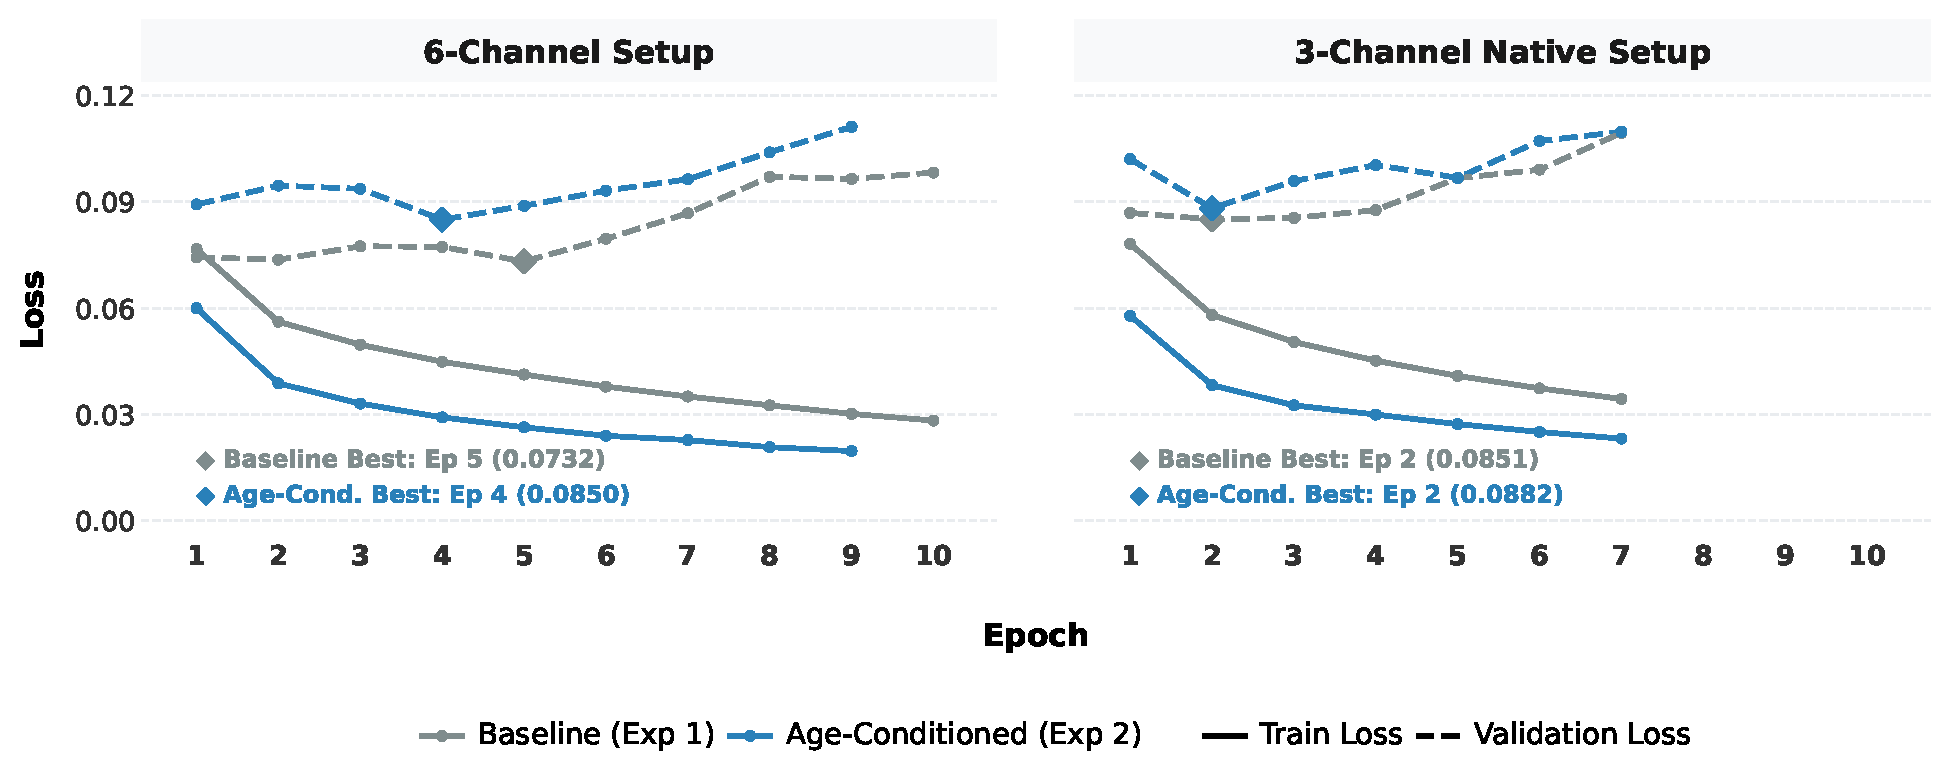
\includegraphics[width=\textwidth]{fig_loss_generalist.pdf}
\caption{\textbf{Training and Validation Loss Curves for Generalist Models (Experiments 1 and 2).} Direct comparison of convergence and generalization across the 6-channel and native 3-channel setups, with diamonds marking the best validation checkpoints. In both architectures, training loss decreases steadily while validation loss reaches its minimum in early epochs before rising due to overfitting, motivating early stopping.}    \label{fig:exp1_exp2_loss}
\end{figure}

\FloatBarrier
\section{Experiment 3: Age-Specific Models}
While the age-conditioned model (Experiment 2) successfully mitigated spatial brittleness and balanced cohort metrics, it still processed all demographics through shared temporal weights. We hypothesized that the generalist model might still be underfitting purely demographic-specific patterns. To test this, we completely partitioned the dataset into the four distinct age cohorts and trained dedicated, age-specific models for each group. 

\subsection{Setup}
We trained each model independently using the optimal hyperparameters we established in the baseline experiment. We employed early stopping based on validation loss to prevent overfitting. As we detailed previously in Section \ref{sec:exp2_data}, the volume of training data varies significantly across the cohorts (ranging from over 167,000 samples for Adults to merely 7,429 for Children). This severe discrepancy naturally influences both the convergence speed and the generalization capabilities of the resulting independent networks.

\subsection{Results and Limitations}
As in the previous experiments, we evaluated the performance of the age-specific models under two spatial resolutions: utilizing the full 6-channel configuration and simulating a modality mismatch by feeding only 3 channels into the 6-channel trained model. Finally, we evaluated natively trained 3-channel models.

\subsubsection*{Full Model (6 Channels)}
By isolating the age groups, the specialized models yielded mixed results when compared to the generalist baseline. We observed the most profound improvement in the Teenagers cohort, where accuracy surged from 66.13\% in the unconditioned baseline model to 83.38\% (Cohen's Kappa was 0.768). The Infants model also saw a slight improvement, achieving an accuracy of 74.87\% compared to the baseline's 73.14\%. 

Conversely, the model trained specifically on the Adults cohort actually saw a slight decrease in accuracy (75.74\% compared to the baseline's 76.76\%), suggesting that the generalist model benefited from the massive aggregate dataset for this dominant group. The Children cohort performed significantly worse than the generalist setups (70.37\% accuracy compared to 76.18\% in the conditioned model). This degradation is directly attributable to the exceptionally small training set for this specific age group, which proved insufficient for an isolated 6-channel model to learn robust stage-discriminative features without overfitting.

\subsubsection*{Robustness to Missing Channels}
To evaluate robustness against sensor loss, we tested the specialized 6-channel models using only 3 channels. Similar to the unconditioned baseline experiment, spatial reduction exposed significant vulnerabilities, though the severity varied substantially by age group. 

The Adults model proved relatively robust, suffering only a moderate drop in accuracy to 73.09\% (down from 75.74\%). The Teenagers model also demonstrated reasonable resilience, dropping to 75.66\%. In stark contrast, the Infants model fell by nearly 11 points to 64.27\%. The most catastrophic failure occurred in the data-starved Children model, where accuracy plummeted to a mere 34.69\% (Cohen's Kappa was 0.188). This demonstrates that without sufficient training volume, an isolated network completely over-leverages highly specific spatial patterns that, when missing, effectively reduce the model's predictions to random guessing.

\subsubsection*{Reduced Channel Model (3 Channels)}
To ascertain whether we could avoid the missing-channel collapse, we natively trained and evaluated age-specific models entirely on the reduced 3-channel setup. Training directly on the restricted spatial resolution successfully restored performance across all cohorts compared to the simulated missing-data scenario.

For Adults, Teenagers, and Infants, the natively trained 3-channel models performed remarkably close to their 6-channel counterparts (achieving accuracies of 75.55\%, 82.61\%, and 73.59\%, respectively). This indicates that we preserve the core sleep staging information even with fewer sensors. 

\begin{table}[ht]
\centering
\caption{\textbf{Age-Specific Model Performance.} This table displays the evaluation metrics for networks trained exclusively on isolated demographic cohorts. It highlights the significant accuracy gains for teenagers, as well as the extreme vulnerability of the children model which we trained on a much smaller dataset when we subjected it to simulated sensor loss.} \label{tab:age_specific_results}
\resizebox{\textwidth}{!}{%
\begin{tabular}{l c c | c c | c c}
\toprule
& \multicolumn{2}{c|}{\textbf{Evaluated on 6 ch}} & \multicolumn{2}{c|}{\textbf{Evaluated on 3 ch (Missing Data)}} & \multicolumn{2}{c}{\textbf{Trained \& Evaluated on 3 ch}} \\
\cmidrule(lr){2-3} \cmidrule(lr){4-5} \cmidrule(l){6-7}
\textbf{Age Group} & \textbf{Accuracy} & \textbf{Kappa} & \textbf{Accuracy} & \textbf{Kappa} & \textbf{Accuracy} & \textbf{Kappa} \\
\midrule
Adults    & 75.74\% & 0.670 & 73.09\% & 0.633 & 75.55\% & 0.668 \\
Teenagers & 83.38\% & 0.768 & 75.66\% & 0.648 & 82.61\% & 0.756 \\
Children  & 70.37\% & 0.573 & 34.69\% & 0.188 & 67.18\% & 0.502 \\
Infants   & 74.87\% & 0.665 & 64.27\% & 0.523 & 73.59\% & 0.648 \\
\bottomrule
\end{tabular}%
}
\end{table}

\FloatBarrier
\section{Experiment 4: Fine-Tuning Pre-Trained Adult Models on Younger Cohorts}

Findings from Experiment 3 highlighted a critical challenge in modeling pediatric and adolescent sleep: extreme data imbalance across demographics. The specialized models for younger cohorts (particularly Children, with only 7,429 training samples) suffered from insufficient data, limiting their ability to learn robust, generalized representations from scratch. To address this, we theorized that we could leverage the vast amount of adult data (over 167,000 samples) to learn foundational sleep features, which we could then adapt to younger demographics.

\subsection{Setup and Methodology}
In this experiment, we employed a transfer learning approach. We utilized both the 6-channel and 3-channel models we trained exclusively on Adults (from Experiment 3) as our base networks. 

We subsequently fine-tuned these pre-trained networks independently on the respective datasets for teenagers, children, and infants. To comprehensively evaluate the models and assess robustness to sensor loss, we evaluated the fine-tuned 6-channel models twice: once on the full 6 channels, and once using only 3 channels to simulate missing data. At the same time, we evaluated the fine-tuned 3-channel models natively on 3 channels. The fine-tuning process retained the optimal hyperparameter configuration we established earlier (learning rate of $5 \times 10^{-5}$, batch size of 16, and dropout of 0.4), utilizing early stopping based on validation loss.

\subsection{Results and Discussion}

Table~\ref{tab:transfer_learning_comparison_all} details the performance of the transfer learning approach across the three evaluation setups. 

\begin{table}[ht]
\centering
\caption{\textbf{Transfer Learning Performance Across Target Demographics.} This table presents the evaluation metrics for each cohort after fine-tuning adult pre-trained base models. It shows that adult priors work better on teenage cohorts which are similar to the adult population and provide regularization that substantially buffers against performance collapse during sensor loss.} \label{tab:transfer_learning_comparison_all}\resizebox{\textwidth}{!}{%
\begin{tabular}{l c c | c c | c c}
\toprule
& \multicolumn{2}{c|}{\textbf{TL (Trained 6ch $\rightarrow$ Eval 6ch)}} & \multicolumn{2}{c|}{\textbf{TL (Trained 6ch $\rightarrow$ Eval 3ch)}} & \multicolumn{2}{c}{\textbf{TL (Trained 3ch $\rightarrow$ Eval 3ch)}} \\
\cmidrule(lr){2-3} \cmidrule(lr){4-5} \cmidrule(l){6-7}
\textbf{Target Age Group} & \textbf{Accuracy} & \textbf{Kappa} & \textbf{Accuracy} & \textbf{Kappa} & \textbf{Accuracy} & \textbf{Kappa} \\
\midrule
Teenagers & 83.63\% & 0.768 & 80.62\% & 0.731 & 82.26\% & 0.751 \\
Children  & 67.22\% & 0.525 & 57.27\% & 0.413 & 69.99\% & 0.559 \\
Infants   & 71.05\% & 0.616 & 63.71\% & 0.515 & 72.41\% & 0.632 \\
\bottomrule
\end{tabular}%
}
\end{table}

\subsubsection*{Overall Performance vs. Training from Scratch}
Contrary to initial expectations, transfer learning did not uniformly improve absolute peak performance compared to the models 
we trained from scratch in Experiment 3. When we evaluated the full 6-channel models, the fine-tuned network for Teenagers achieved a 
marginal improvement, reaching 83.63\% compared to its from-scratch counterpart (83.38\%). However, the fine-tuned models for Children
(67.22\%) and Infants (71.05\%) underperformed their from-scratch baselines (70.37\% and 74.87\%, respectively). This suggests that
while adult priors provide a strong initialization that transfers effectively to adolescents, heavily anchoring the weights in adult
spatial-temporal features may slightly restrict the model from perfectly converging on the more distinct, native EEG morphologies of
early developmental pediatric cohorts. This is somewhat sensible as sleep patterns go through quite large changes, from birth and into adulthood. \todo{ukradeno iz tvojega komentarja :) se mi zdi da je to samo po sebi dovolj dobra hipoteza.}

\subsubsection*{Mitigating Catastrophic Degradation}
Where transfer learning demonstrated profound clinical value was in improving robustness for data-starved demographics. In Experiment 3, the from-scratch 6-channel Children model suffered a catastrophic collapse to 34.69\% accuracy when we evaluated it on 3 channels. In stark contrast, the transfer-learned 6-channel model maintained a much more stable 57.27\% accuracy under the exact same missing-data simulation. By grounding the network in generalized spatial priors we learned from the massive adult dataset, the fine-tuned model avoids over-leveraging spatial correlations, significantly buffering against random guessing during sensor loss.

\subsubsection*{3-Channel Transfer Learning as Regularization}
Interestingly, for the Infant cohorts, fine-tuning the natively 3-channel adult model yielded better overall accuracy (72.41\%) than fine-tuning the full 6-channel model (71.05\%). This reinforces a finding we observed in Experiment 3: a reduced spatial resolution effectively acts as a form of architectural regularization. When we adapt learned weights across demographic domains, restricting the spatial feature space prevents the transfer of overly rigid, adult-specific spatial patterns, ultimately improving generalization on the younger target domains.

\begin{figure}[p]
    \centering
    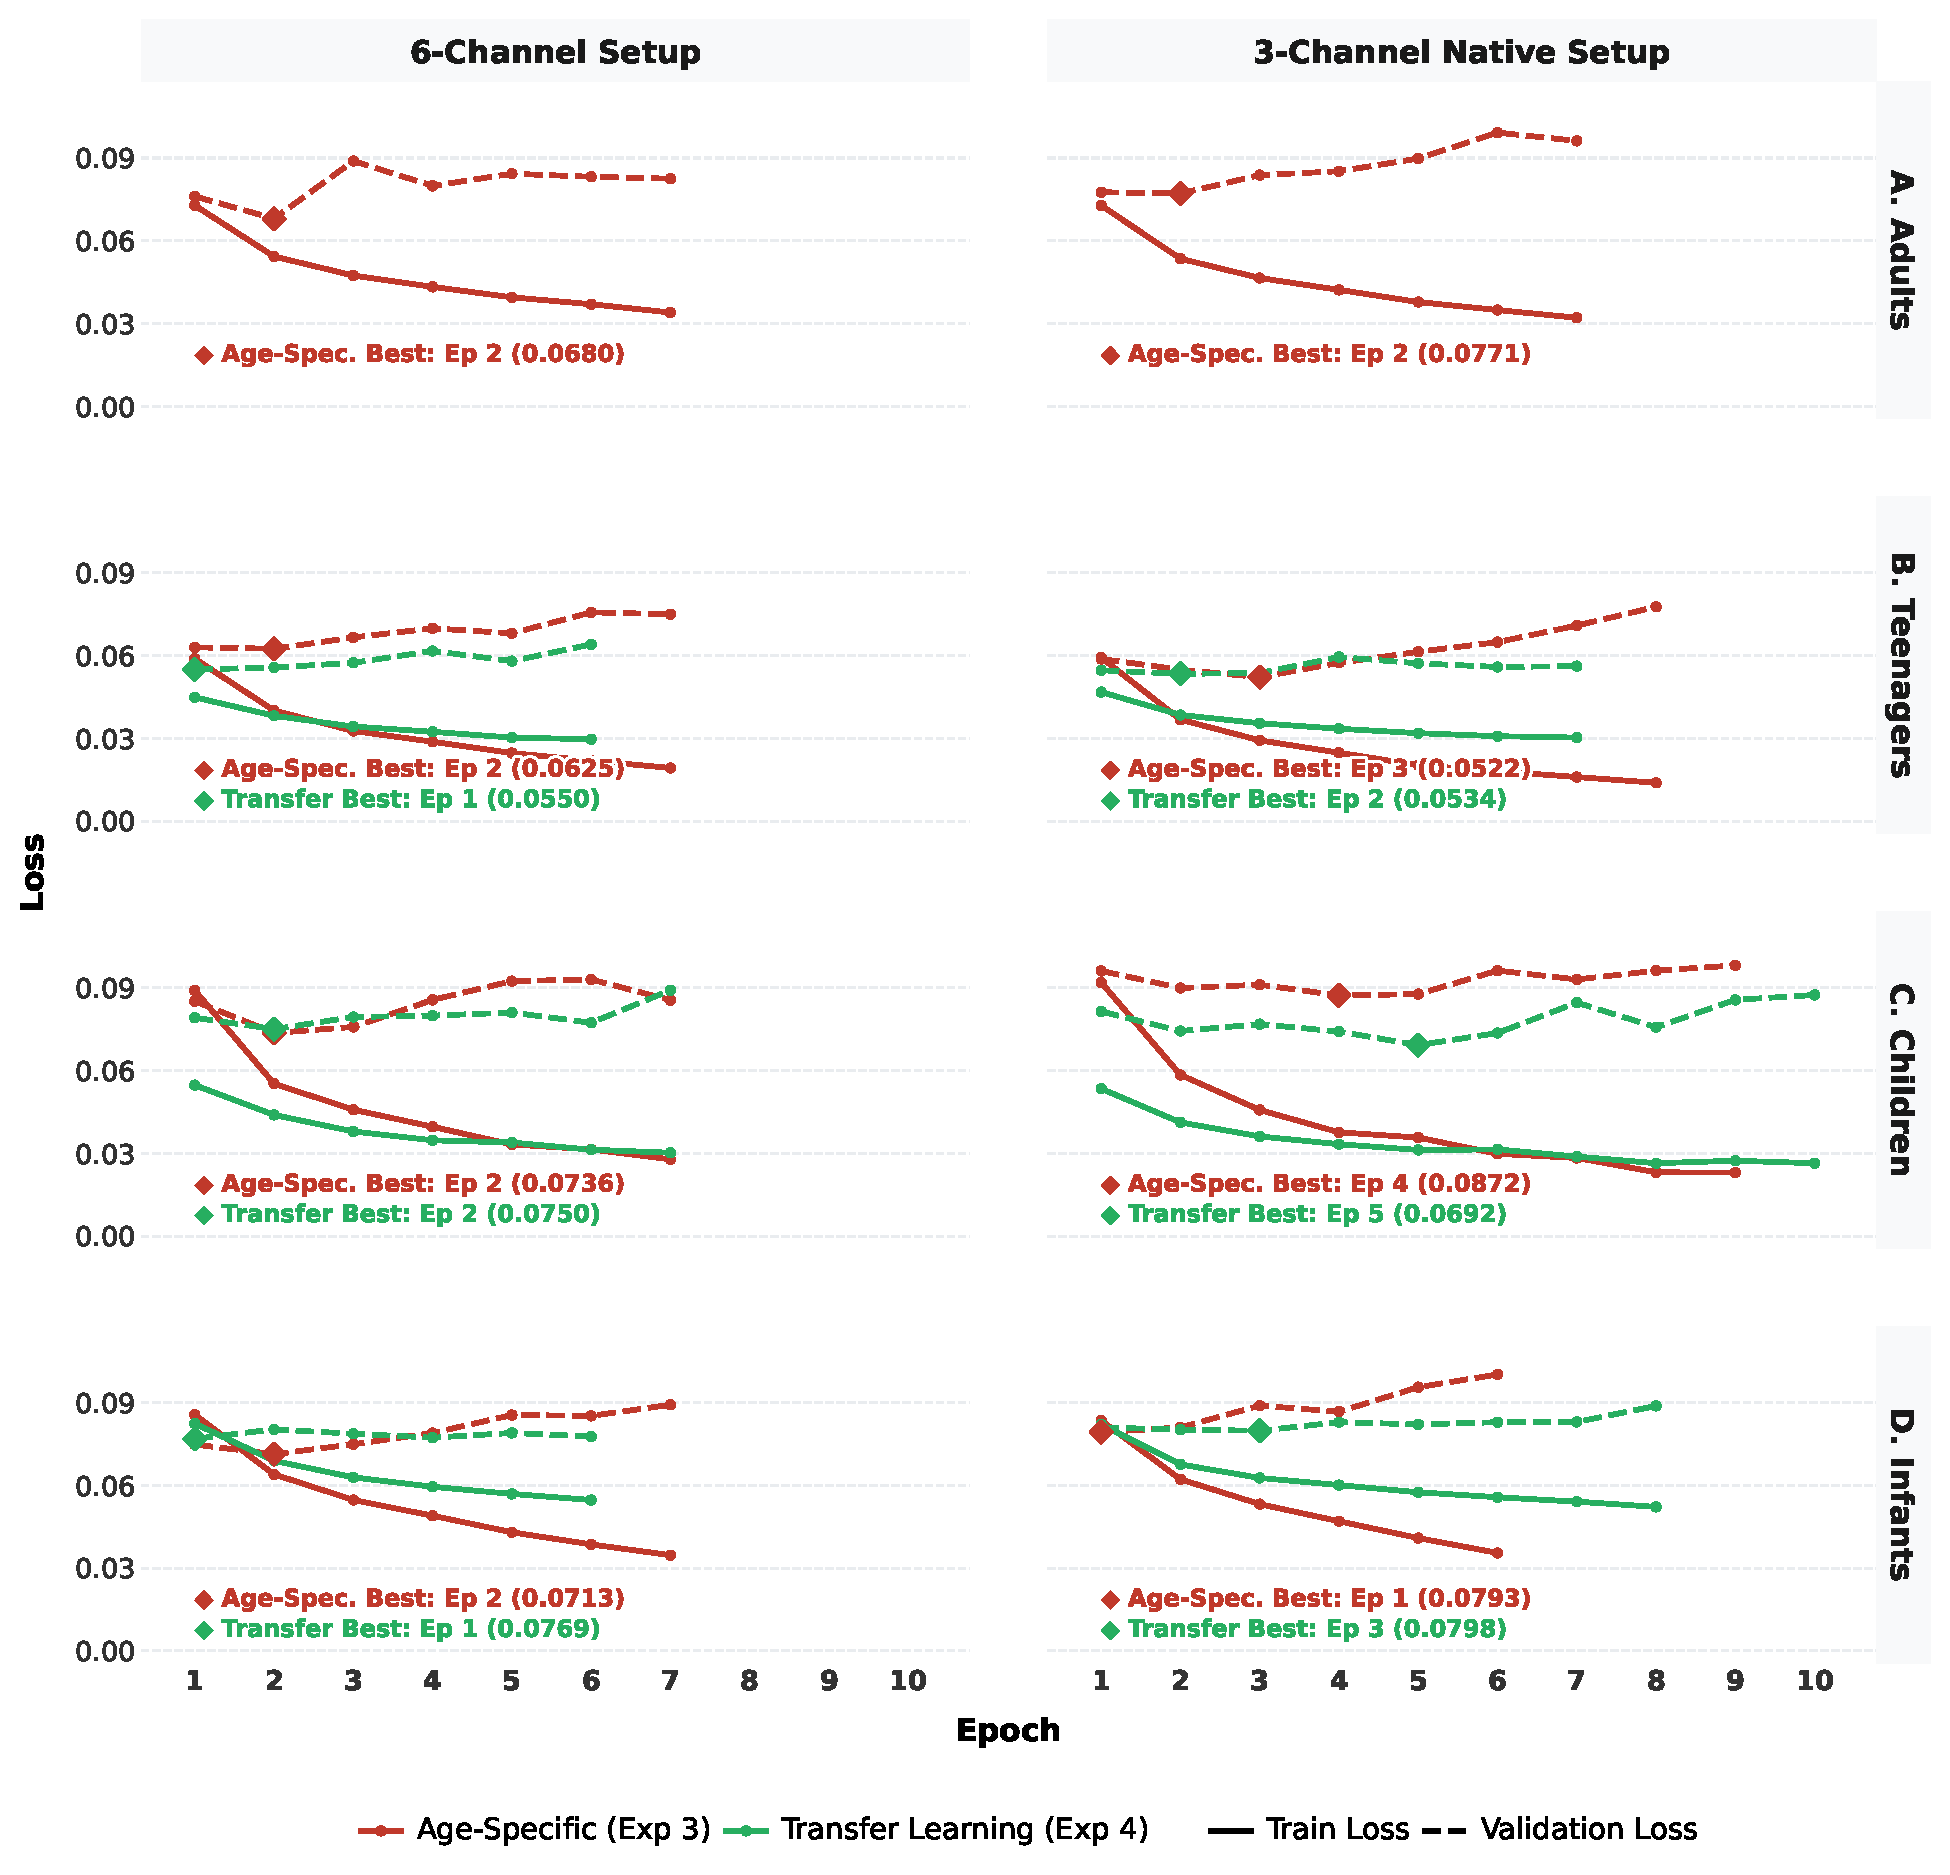
\includegraphics[width=\textwidth]{fig_loss_age_vs_tl.pdf}
    \caption{\textbf{Training and Validation Loss Curves for Age-Specific and Transfer Learning Models (Experiments 3 and 4).} Fine-tuning adult priors (green) yields lower initial training loss across younger cohorts compared to training from scratch (red).}
    \label{fig:exp3_exp4_loss}
\end{figure}

\FloatBarrier

\section{Experiment 5: Comparison with an Established Classification Model (YASA)} \label{sec:yasa_comparison}
YASA (Yet Another Spindle Algorithm) \cite{VallatWalker2021} is a popular, publicly available open-source tool for automated sleep staging. In this section, we evaluate how our proposed architectures compare to this highly established, off-the-shelf model. 

\subsection{Setup and Methodology}
We evaluated the YASA model on a specific subset of our data due to differing input requirements.
While our proposed models independently process isolated 30-second
multi-channel spectrograms, YASA operates on a single EEG channel and relies on temporal context across
surrounding epochs, requiring continuous sleep recordings as input. Our model is therefore more flexible in its input requirements,
as we can always compute spectrograms from raw EEG recordings, whereas we cannot reconstruct raw EEG from spectrograms due to the loss of phase information.
We sourced all recordings used for this comparative baseline from the NCH Sleep DataBank \cite{NCHSleep}.

Furthermore, YASA's feature extraction incorporates patient sex as a demographic input. Because explicit sex metadata was unavailable for this specific evaluation subset, we adopted an optimistic evaluation protocol: we evaluated each recording twice—once configured as male and once as female—and retained the higher-performing outcome. This ensures an upper-bound estimate of YASA's predictive capability on our dataset.

We calculated the accuracy of the YASA model for each age group, reporting results as the mean accuracy across the individual recordings alongside the standard deviation. We summarize the details of this evaluation subset—including the number of full recordings and total extracted 30-second epochs per demographic—as well as the resulting model performance, in Table~\ref{tab:yasa_results}.

\begin{table}[ht]
\centering
\caption{\textbf{YASA Benchmark Performance Across Age Cohorts.} This table summarizes the recording counts, total epoch volumes, and mean classification accuracy for the off-the-shelf YASA model on the NCH Sleep DataBank subset. It reveals a steep developmental degradation, demonstrating that adult-centric staging features struggle to generalize down to infant cohorts.}
\label{tab:yasa_results}
\begin{tabular}{l c c c}
\toprule
\textbf{Age Group} & \textbf{Recordings ($n$)} & \textbf{Epochs} & \textbf{Accuracy (Mean $\pm$ SD)} \\
\midrule
Adults    & 55 & 52,966 & 67.60\% $\pm$ 10.51\% \\
Teenagers & 87 & 85,887 & 65.39\% $\pm$ 15.73\% \\
Children  & 64 & 65,877 & 60.94\% $\pm$ 13.18\% \\
Infants   & 66 & 66,594 & 44.96\% $\pm$ 13.92\% \\
\bottomrule
\end{tabular}
\end{table}

\subsection{Results and Discussion}
The evaluation reveals a clear developmental trend: even under an upper-bound evaluation setup, YASA performs reasonably well on adult data but suffers severe performance degradation on younger cohorts. For the \textbf{Adults} cohort, YASA achieved an average accuracy of 67.60\%. While this serves as a solid baseline, it underperforms compared to our proposed baseline network (76.76\% in Experiment 1) and our age-conditioned model (75.36\% in Experiment 2). 

As the demographic age decreases, YASA's performance gap widens considerably. It achieved 65.39\% for \textbf{Teenagers} and 60.94\% for \textbf{Children}. In stark contrast, our natively trained age-specific models (Experiment 3) reached up to 83.38\% for Teenagers, and our age-conditioned model (Experiment 2) achieved 76.18\% for Children.

We observe the most catastrophic failure of the established model in the \textbf{Infants} cohort, where YASA's accuracy plummets to 44.96\%. This sharp decline perfectly illustrates the core problem our work addresses: researchers heavily optimize traditional single-channel sleep staging algorithms on adult populations. Consequently, their hand-crafted features and adult-centric temporal priors completely fail to generalize to pediatric cohorts. By contrast, our approaches—whether via explicit age-conditioning (73.79\%) or age-specific model partitioning (74.87\%)—successfully captured these unique developmental patterns, outperforming the established YASA model by nearly 30 percentage points for infants.

This performance drop occurs because developers of YASA explicitly developed and trained YASA on adult demographics, meaning it expects fully mature sleep architectures. Thus, we expect that YASA's adult-centric parameters naturally struggle to accurately interpret the sleep data of younger cohorts.

\FloatBarrier
\begin{landscape}
\begin{figure}[p]
    \centering
    % Constrain the HEIGHT so ~30% of the vertical page space is left for the caption
    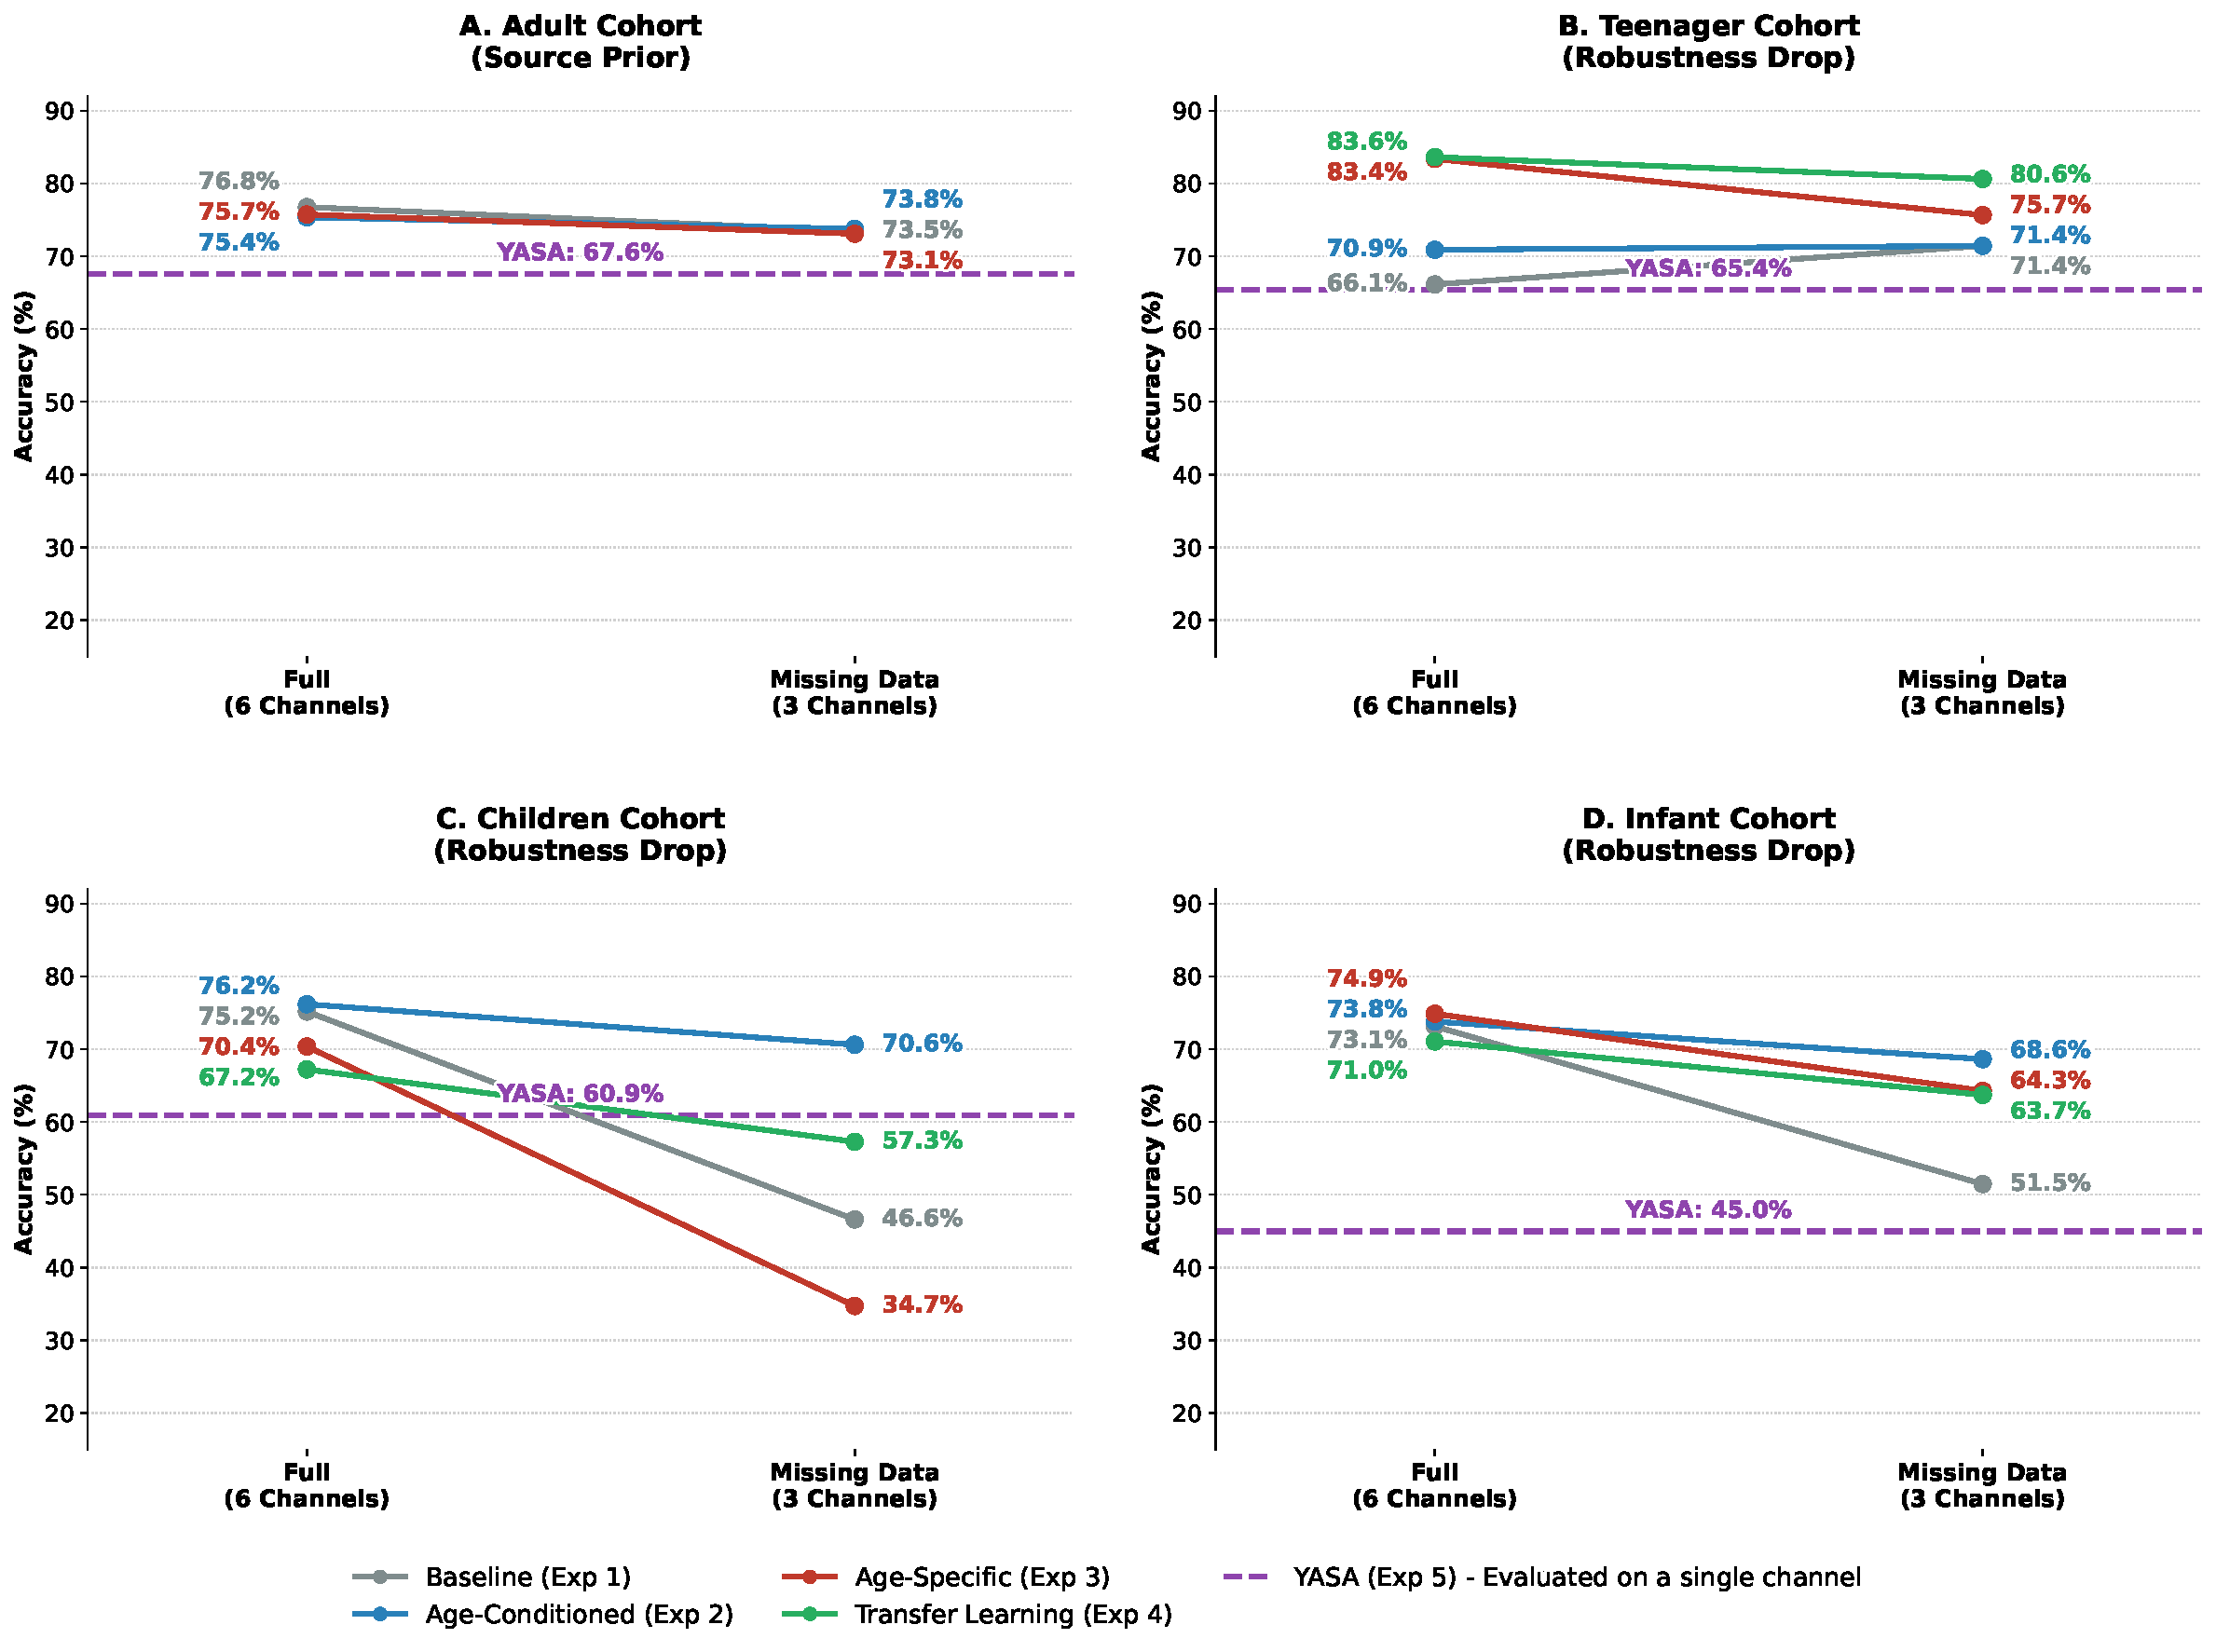
\includegraphics[height=0.98\textheight, keepaspectratio]{experiments_slope_chart.pdf}
    \vspace{0.5cm}
    \caption{\textbf{Cross-Experiment Comparison and Sensor Loss Robustness.}  This slope chart visualizes accuracy degradation when models encounter missing channels at inference. It shows how demographic conditioning and transfer learning buffer younger cohorts against sensor loss.}
    \label{fig:overall_comparison}
\end{figure}
\end{landscape}

\section{Age-Routed Sleep Staging Framework}
\label{sec:routing_framework}

The preceding evaluations (Experiments 1 through 4) demonstrate that no single architectural setup achieves optimal performance
and robustness across all developmental stages. While adult and adolescent recordings benefit from broad spatial configurations
and transfer learning, dedicated age-specific networks best capture infant sleep, and the data-starved children
cohort requires the regularization that demographic conditioning provides.

We used these findings to develop a simple, age-routed
inference framework. Instead of relying on a specific architecture, this framework dynamically selects and deploys
the optimally performing model configuration we found in previous experiments based on the patient's biological age 
at the time of the recording. 

When we provide a new recording, the pipeline extracts the patient's age and routes the sequence of 30-second
EEG spectrograms to one of four specialized, pre-trained networks:
\begin{itemize}
    \item \textbf{adults (Age $\geq$ 18 years):} we process the sequence with the standard generalist baseline model (Experiment 1), which benefits from the massive dataset,
    \item \textbf{teenagers (12 to 18 years):} we route it to the fine-tuned transfer learning model (Experiment 4), which successfully adapts adult spatial priors to adolescent waveforms,
    \item \textbf{children (2 to 12 years):} we handle it with the age-conditioned model (Experiment 2), which requires an explicit demographic embedding tensor,
    \item \textbf{infants ($<$ 2 years):} we evaluate it using the natively trained age-specific network (Experiment 3), which best captures the highly distinct EEG patterns unique to early pediatric development.
\end{itemize}
If the patient's age is missing, the router falls back to the baseline model, which was trained on all age groups.

Each demographic cohort exposes both the full 6-channel variant and the natively trained 3-channel variant evaluated earlier in this chapter. 
If a recording contains more than 3 channels, the framework selects the 6-channel variant. If it contains 3 or fewer channels, it automatically
routes the input to the natively trained 3-channel variant. Should a recording still differ from the selected variant's expected channel count
(for example, 1 or 2 channels routed to a 3-channel model), the pipeline zero-pads the missing dimensions.

Prior to inference, each recording is standardized using the exact training-set mean and standard deviation associated with the
selected cohort and channel variant. When ground-truth stage annotations are available the framework automatically computes per-recording and
aggregate evaluation metrics (accuracy, Cohen's Kappa, macro F1 and confusion matrices). By harmonizing these architectural and spatial-resolution
strategies into a single programmatic interface, the framework maximizes predictive accuracy and clinical robustness across all studied developmental stages of this thesis.
